% case name
\chapter{trigrid\_mail\_tot}
%
%
% - Purpose & Description:
%     These first two parts give reader short details about the test case,
%     the physical phenomena involved, the geometry and specify how the numerical solution will be validated
\section{Purpose}
This example illustrates the conversion from a mesh file generated with
TRIGRID to a Serafin file.
%
\section{Description}
The computation deals with the elimination of the overstressed triangles within
the entire mesh.\\
At any rate, the bathymetry found in the TRIGRID file is used to inform the
variable BOTTOM of the geometry file generated by \stbtel. In the same way, the
colour codes located along the boundaries points during the TRIGRID session
allow \stbtel to create a boundary condition file which makes appear a boundary
with a imposed flowrate on the left side and a imposed water level on the right
side.

%
% - Physical parameters:
%     This part specifies details all the physical parameters
%\subsection{Physical parameters}
%
% Experimental results (if needed)
%\subsection{Experimental results}
%
% bibliography can be here or at the end
%\subsection{Reference}
%
% Section for computational options
%\section{Computational options}
%
% - Mesh:
%     This part describes the mesh used in the computation
%\subsection{Mesh}
%
% - Initial and boundary conditions:
%     This part details both initial and boundary conditions used to simulate the case
%\subsection{Initial and boundary conditions}
%
% - Numerical parameters:
%     This part is used to specify the numerical parameters used
%     (adaptive time step, mass-lumping when necessary...)
%\subsection{Numerical parameters}
%
% - Results:
%     We comment in this part the numerical results against the reference ones,
%     giving understanding keys and making assumptions when necessary.
\section{Results}
The resulted mesh is shown in figure \ref{fig:trigridmailtot:mesh} and the
bathymetry in figure \ref{fig:trigridmailtot:bathy}:
\begin{figure}[H]%
\begin{center}
%
  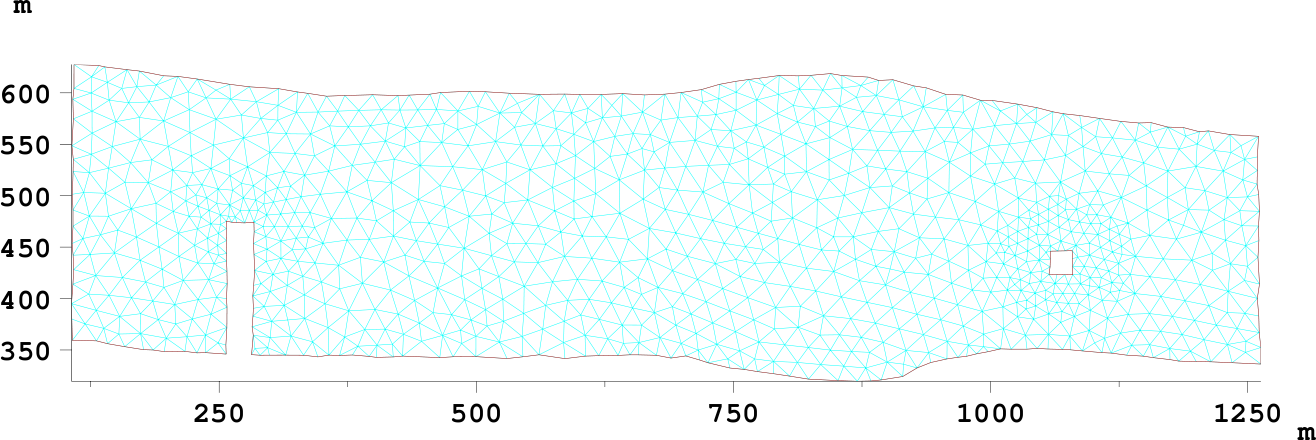
\includegraphics[width=0.9\textwidth]{mesh}
%
\end{center}
\caption
{The mesh}
\label{fig:trigridmailtot:mesh}
\end{figure}
%
\begin{figure}[H]%
\begin{center}
%
  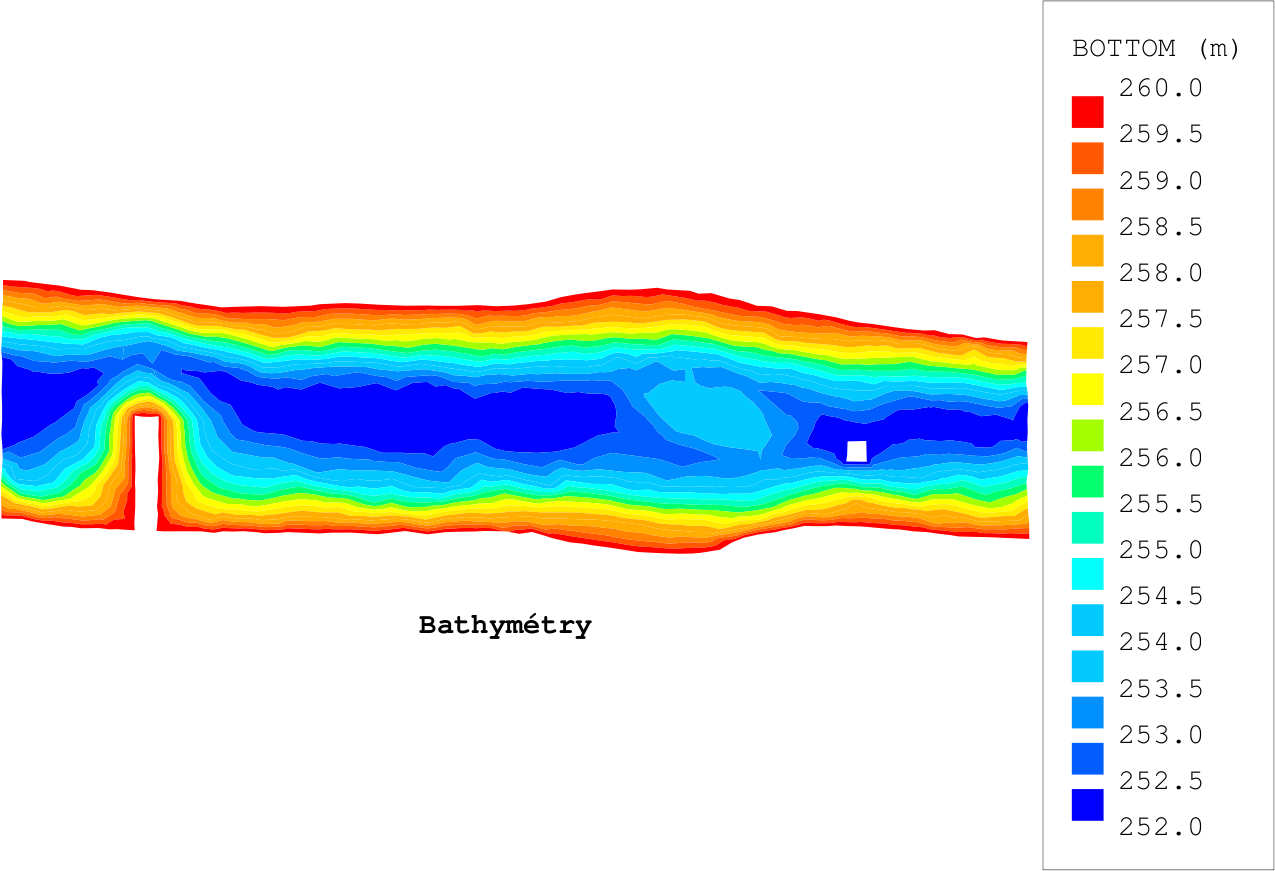
\includegraphics[width=0.9\textwidth]{bathy}
%
\end{center}
\caption
{The bathymetry}
\label{fig:trigridmailtot:bathy}
\end{figure}
%
% bibliography
%\section{Reference}
